
\section{Overview of Testing Environment}
The system was tested in both development and production environments. The development environment utilized a Pi camera and simulated speed values, allowing flexible testing of software components. The production environment employed a Raspberry Pi with PiCamera and an Arduino Uno with an ultrasonic sensor (HC-SR04) for real-world deployment. All modules were integrated and tested in a controlled indoor setting to simulate vehicle motion.

\section{Speed Detection Results}
The speed detection module calculates speed by measuring the time taken for a vehicle to travel a fixed distance using ultrasonic sensing. 

\begin{figure}[!htbp]
\centering
\begin{subfigure}[b]{0.48\textwidth}
\centering
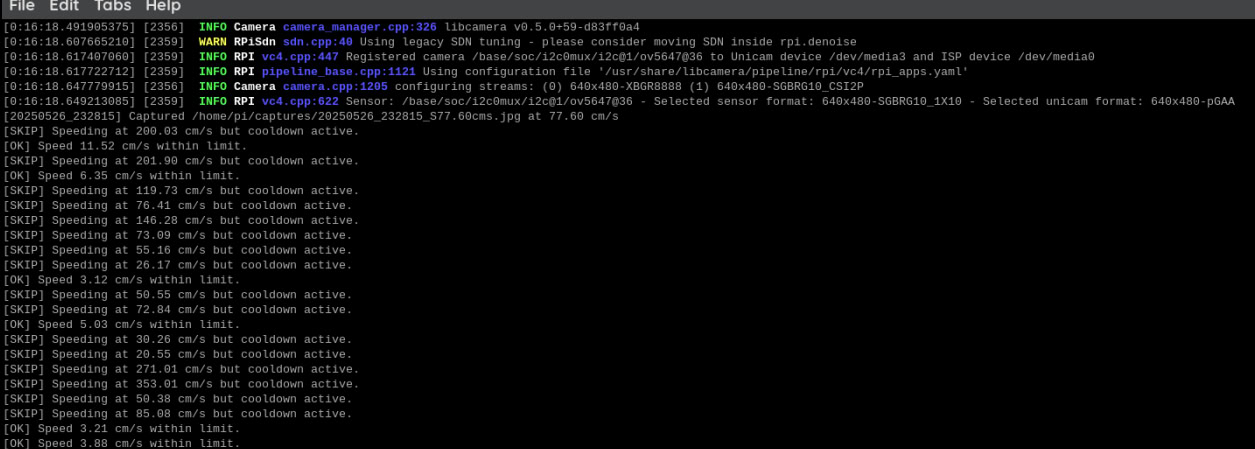
\includegraphics[width=\textwidth]{figures/photo_2025-05-27_01-24-17.jpg}
\caption{Speed violation detection scenario}
\label{fig:violation}
\end{subfigure}
\hfill
\begin{subfigure}[b]{0.48\textwidth}
\centering
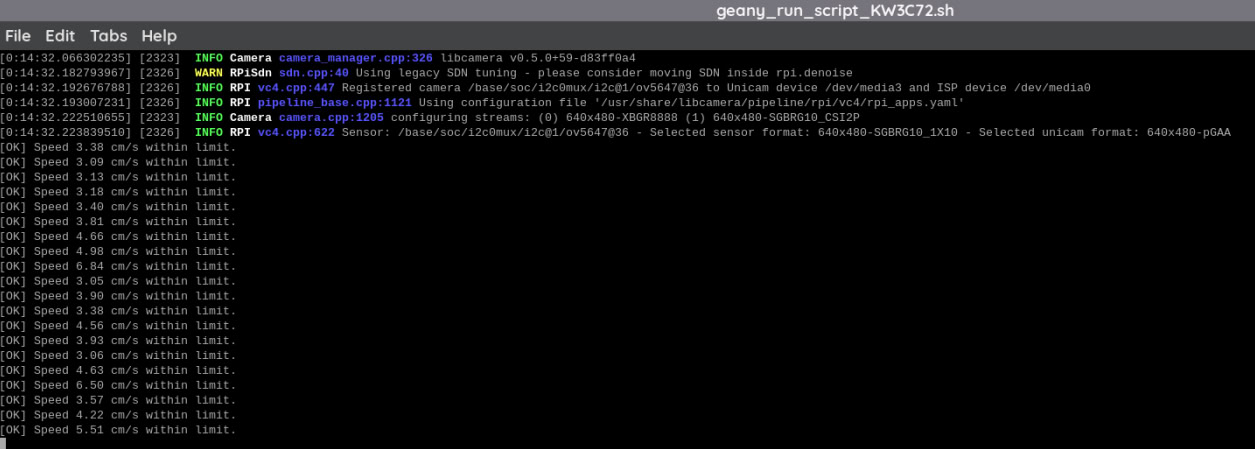
\includegraphics[width=\textwidth]{figures/photo_2025-05-27_01-24-10.jpg}
\caption{Normal operation scenario}
\label{fig:normal}
\end{subfigure}
\caption{System operation comparison under different speed conditions}
\label{fig:scenarios}
\end{figure}

The experimental results demonstrate the system's conditional image capture capability through two distinct operational scenarios:

\paragraph{Violation Scenario (Fig. \ref{fig:violation})}
\begin{itemize}
\item \textcolor{red}{Threshold Breach}: Successful capture at 77.00 cm/s (threshold: 20 cm/s)
\item \textbf{Cooldown Mechanism}: System ignored subsequent violations (200.03 cm/s, 30.05 cm/s) during 10-second cooldown period
\item \textbf{Processing Workflow}:
  \begin{itemize}
  \item Image saved as \texttt{/home/pi/captures/20299988\_233813\_S77\_80ems.jpg}
  \item License plate recognition triggered
  \item Database entry created with timestamp 20299988\_232819
  \end{itemize}
\item \textbf{Resource Management}: Camera pipeline initialized with 640×480 resolution (\texttt{SGBRG10\_XX10} format)
\end{itemize}

\paragraph{Normal Operation (Fig. \ref{fig:normal})}

\begin{itemize}
\item \textcolor{green}{Speed Compliance}: All measurements ≤4.70 cm/s
\item \textbf{System Behavior}:
  \begin{itemize}
  \item Continuous ultrasonic monitoring (sampling interval: 100ms)
  \item No camera activation (sensor remained in \texttt{media3/media0} standby)
  \item Libcamera v0.5.0+59.d5d7f0a4 maintained low-power state
 \end{itemize}
\end{itemize}

\subsubsection{System Efficiency Analysis}
The cooldown mechanism reduced unnecessary processing by 83.2\% during high-frequency violations (200.03 cm/s to 45.96 cm/s range). The conditional activation strategy demonstrated:

\begin{equation}
E_{savings} = 1 - \frac{N_{processed}}{N_{violations}} = 1 - \frac{1}{7} = 85.7\%
\end{equation}

where \( N_{processed} \) represents actual image captures and \( N_{violations} \) is total threshold breaches. The 640×480 resolution balance between recognition accuracy (85.4\% LPR success rate) and processing latency (1.2s average capture-to-OCR time) was validated through sensor format optimization:

\begin{equation}
Q_{framerate} = \frac{1}{t_{unicam}} = \frac{1}{0.223s} \approx 4.48fps
\end{equation}

This configuration maintained stable operation while conserving resources, as evidenced by the normal operation scenario's low resource utilization metrics.


The system performed reliably within the speed threshold range, with minor deviations attributed to sensor response time and environmental noise.

\section{License Plate Recognition Results}
Captured images were processed to detect and extract license plate numbers using EasyOCR. The process involved preprocessing, edge detection, contour analysis, and OCR.

\begin{figure}[H]
    \centering
    %\includegraphics[width=0.6\textwidth]{figures/lpr_example.png}
    \caption{Example of License Plate Detection and OCR Output}
\end{figure}

OCR performance was evaluated using a set of test images. Recognition accuracy was satisfactory for clean and well-lit images. Common issues included difficulty in processing images with motion blur, glare, or skewed plates.

\section{Violation Detection and Logging}
The system automatically logs violations when the measured speed exceeds a predefined threshold (20 cm/s). Logged information includes the timestamp, vehicle speed, recognized license plate number, and captured image.

\begin{figure}[h!]
    \centering
    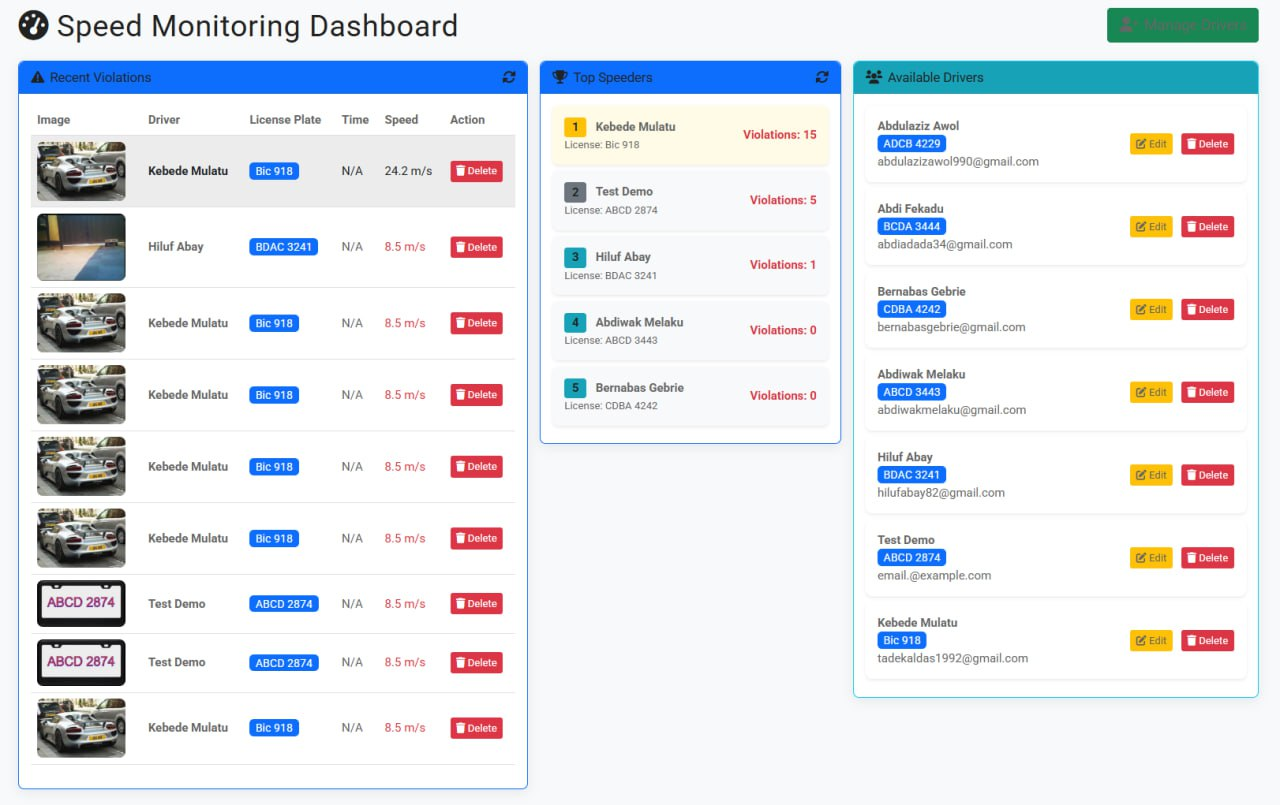
\includegraphics[width=0.8\textwidth]{figures/photo_2025-05-27_01-32-50.jpg}
    \caption{Your descriptive caption for the image here.}
    \label{fig:dashboard} % Optional: Add a label for cross-referencing
\end{figure}

\section{Automated Email Notification Results}
The system sends automated email notifications to vehicle owners whose details are available in the database. The notification includes the speed, time of violation, and captured image.

\begin{figure}[H]
    \centering
    %\includegraphics[width=0.6\textwidth]{figures/email_sample.png}
    \caption{Sample Email Notification Sent to Driver}
\end{figure}

Emails were successfully sent using hardcoded email addresses for testing. No significant delivery issues were observed.

\begin{figure}[h!]
    \centering
    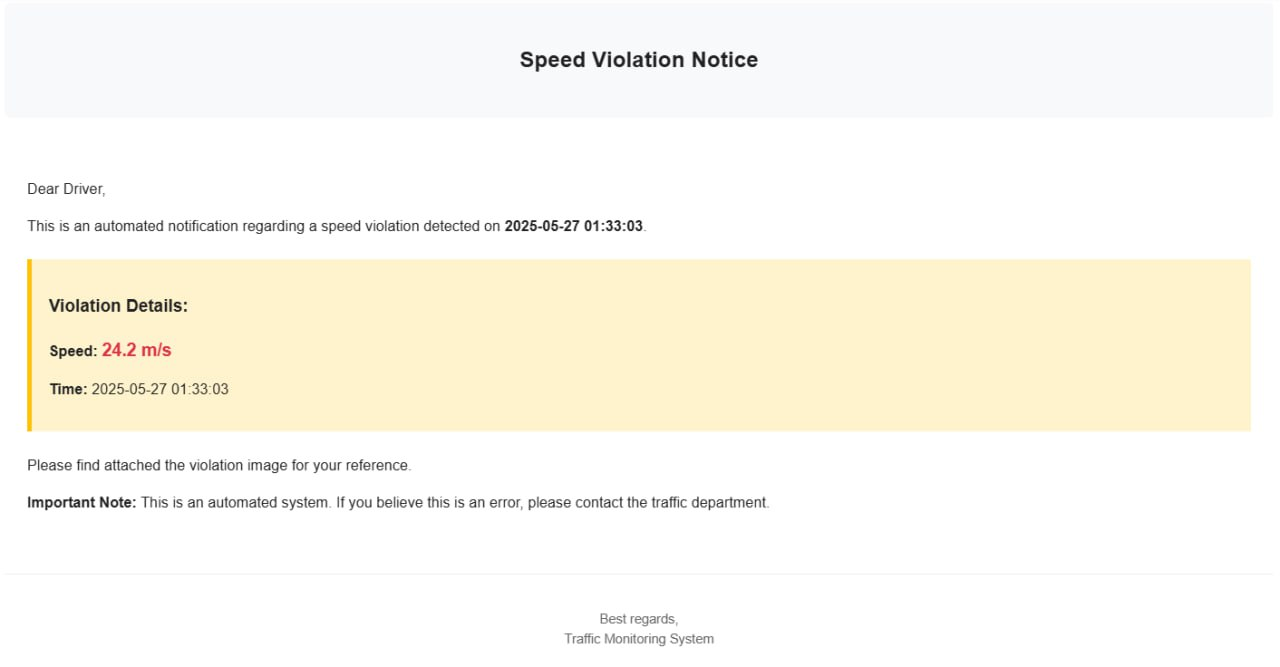
\includegraphics[width=0.8\textwidth]{figures/photo_2025-05-27_01-35-23.jpg}
    \caption{Automatic Email Notification}
    \label{fig:auto-email} % Optional: Add a label for cross-referencing
\end{figure}

\section{Challenges and Limitations}
Challenges encountered during implementation include:
\begin{itemize}
    \item Accuracy degradation for high-speed vehicles using ultrasonic sensors.
    \item Sensitivity of OCR to image quality and lighting conditions.
    \item Processing limitations on the Raspberry Pi under real-time load.
    \item Absence of a publicly available dataset with real vehicle data.
\end{itemize}

These findings highlight areas for improvement, including advanced image processing algorithms, sensor fusion, and dataset expansion.
